\chapter{Calculating Homology and Homotopy}
\label{chap:matint}
\vspace*{-0.9cm}

% \startcontents[chapters]
% \printcontents[chapters]{}{1}{}

\section{Group Theory: The theoretical minimum}
Unfortunately, we need some quite abstract concepts from group theory to understand how to calculate fundamental groups effectively. I will try to keep it at an absolute minimum, just enough to understand the fundamental theorem of this section.
Our goal is to define the amalgamation of two groups. We start with a construction:
Begin with a set $S$ of $n$ letters $\{s_1, \dots, s_n\}$ and add their formal inverse to this set, so we get $\{s_1, s_1^{-1}, \dots, s_n, s_n^{-1}\}$. Now add all possible words you get by arranging those $2n$ letters freely. You are not allowed to permute, so $s_1s_2 \neq s_2s_1$. You are allowed to add a letter multiple times, like $s_1 s_1 s_1 s_2 s_4 s_1 = s_1^4 s_2 s_4 s_1$ is a word. The set obtained in this way is denoted $\mathcal{F}_n$. Define a group operation on those words by just writing them left to right as one word, e.g. on $\mathcal{F}_3$ we could write $$aba \circ cac = abacac.$$ Define the group inverse of $s_i$ as the formal inverse $s_i^{-1}$ such that one can cancel adjacent inverse letters in words, e.g. $abaa^{-1} = ab$. But note that $aba^{-1}$, for example, cannot be simplified. The neutral element is the empty word. Now reduce all words as far as possible, i.e. cancel all adjacent inverses. This defines a group structure on $\mathcal{F}_n$ and we call $\mathcal{F}_n$ the \textbf{free group on $n$ generators}.
\begin{remark}
    As far as groups can be nice, free groups are the exact opposite of a nice group: Even the free group on one generator is infinitely big as it contains all exponents of $a$. Also, for $n>2$ it is never abelian.
\end{remark}
Interesting about free groups is that they can be used to smash two groups together into a new group without caring about how the two groups interact with each other.
\begin{definition}[Free Product]
    \marginnote{This means that we just form words with elements in $G$ and $H$, treating those simply as letters. We allow absolutely no interaction between $G$ and $H$ in the free product, we can only reduce inside of $G$ and inside of $H$, e.g. $hh'ghg'=h''ghg$ where $h\circ h' = h''$ in $H$.}
    Let $G,H$ be two groups. The free product $G \star H$ is defined to be the free group generated by all elements of $G$ and $H$ after performing the following reductions:
    \begin{itemize}
        \item Remove any instance of the identity element of $G$ or $H$.
        \item Replace any pairs of the form $g_i g_j$ by their product in $G$ and any elements of the form $h_i h_j$ by their product in $H$.
    \end{itemize}
\end{definition}
We have one big problem: Given two or even more groups and forming their free product, how do we keep track what can actually be reduced in each of the factors and what not? We need a nice, concise notation to keep track of words and relations. 
Take a set of letters $\{a_1, \dots, a_n\}=:S$ and denote by $\tilde{S}$ the set of all letters and their formal inverses. Let $R$ be a set consisting of certain words of the letters in $\tilde{S}$. Define 
$$ \langle S \mid R \rangle$$
to be a quotient of the free group $\mathcal{F}_n$ where all words in $R$ are allowed to be reduced.
\begin{definition}[Presentation]
    Let $G$ be a group. If there exist some $S$ and $R$ as above such that $$G \cong \langle S \mid R \rangle,$$ we call $\langle S \mid R \rangle$ a \textbf{presentation} of $G$. The set $R$ is called \textbf{relation set}.
\end{definition}
\begin{eg}
    \marginnote{Note that presentations are non-unique. It is even worse: Given a finitely generated group $G$ and two words in the letters of $G$, it is algorithmically indecidable whether they represent the same element of $G$ or not. This is the famous \emph{word problem}.}
    \begin{itemize}
        \item The easiest one is $\mathcal{F}_n \cong \langle \{a_1, \dots, a_n\} \mid \emptyset \rangle$. There are no relations.
        \item We can now attack our problem: Let $G \cong \langle S_G \mid R_G \rangle$ and $H \cong \langle S_H \mid R_H \rangle$ be presentations of $G$ and $H$. Then $$G \ast H \cong \langle S_G \cup S_H \mid R_G \cup R_H \rangle $$ is a presentation of the free product of $G$ and $H$.
        \item The integers have presentation $\langle a \mid \emptyset \rangle$ and are hence isomorphic to $\mathcal{F}_1$.
        \item The cyclic groups have presentation $\mathbb{Z} / n \mathbb{Z} \cong \langle a \mid a^n\rangle$.
    \end{itemize}
\end{eg}
Almost done! We have everything to define the amalgamated free product.
\begin{definition}[Free Product with Amalgamation]
    \marginnote{This seems more abstract than it actually is: We have maps $H \to G_i$. For simplicity, assume they are injective, so they identify some part of $G_i$ with $H$. Then we take the free product of $G_1$ and $G_2$ but we make sure that the part of $G_1$ we identified with $H$ agrees with the counterpart in $G_2$. That is all there is to this construction.}
    Given three groups $G_1,G_2,H$ with presentations $\langle S_{G_i} \mid R_{G_i} \rangle, \langle S_H \mid R_H \rangle$ and two group homomorphisms $\iota_i: H \to G_i$, we define the \textbf{free product of $G_1$ and $G_2$ amalgamated with $H$} as the group 
    \begin{equation}
        G_1 \star_H G_2 := \langle S_{G_1} \cup S_{G_2}\mid R_{G_1}, R_{G_2}, \forall h \in H: \iota_1(h)=\iota_2(h)\rangle.
    \end{equation}
\end{definition}
And with this, we do some interesting stuff.
\section{The Theorem of Seifert-van Kampen}
We want to calculate $\pi_1$ under some reasonable conditions on our topological space. The idea we follow here is to split the space into easier spaces which we understand well to obtain $\pi_1$ of the full space. This will prove to be especially useful for top. spaces given as fundamental diagrams, i.e. "glueing squares".
\begin{theorem}[Seifert-van Kampen]
    Let $(X, \mathcal{T})$ be a path-connected top. space, $X= X_1 \cup X_2$ for some $X_1, X_2 \in \mathcal{T}$ and $x_0 \in X_0 := X_1 \cap X_2$. Furthermore, let $X_0, X_1$ and $X_2$ be also path-connected. Then there is an isomorphism of fundamental groups:
    \begin{equation}
        \pi_1(X_1,x_0) \star_{\pi_1(X_0,x_o)} \pi_1(X_2,x_0) \cong \pi_1(X, x_0).
    \end{equation}
\end{theorem}
The nice thing about this theorem is that we can prove many things with nice diagrams. The not so nice part is that you really need all the assumptions. This theorem is horribly wrong if one of those spaces is not path-connected or open.
\begin{eg}
        \begin{marginfigure}
            \centering
        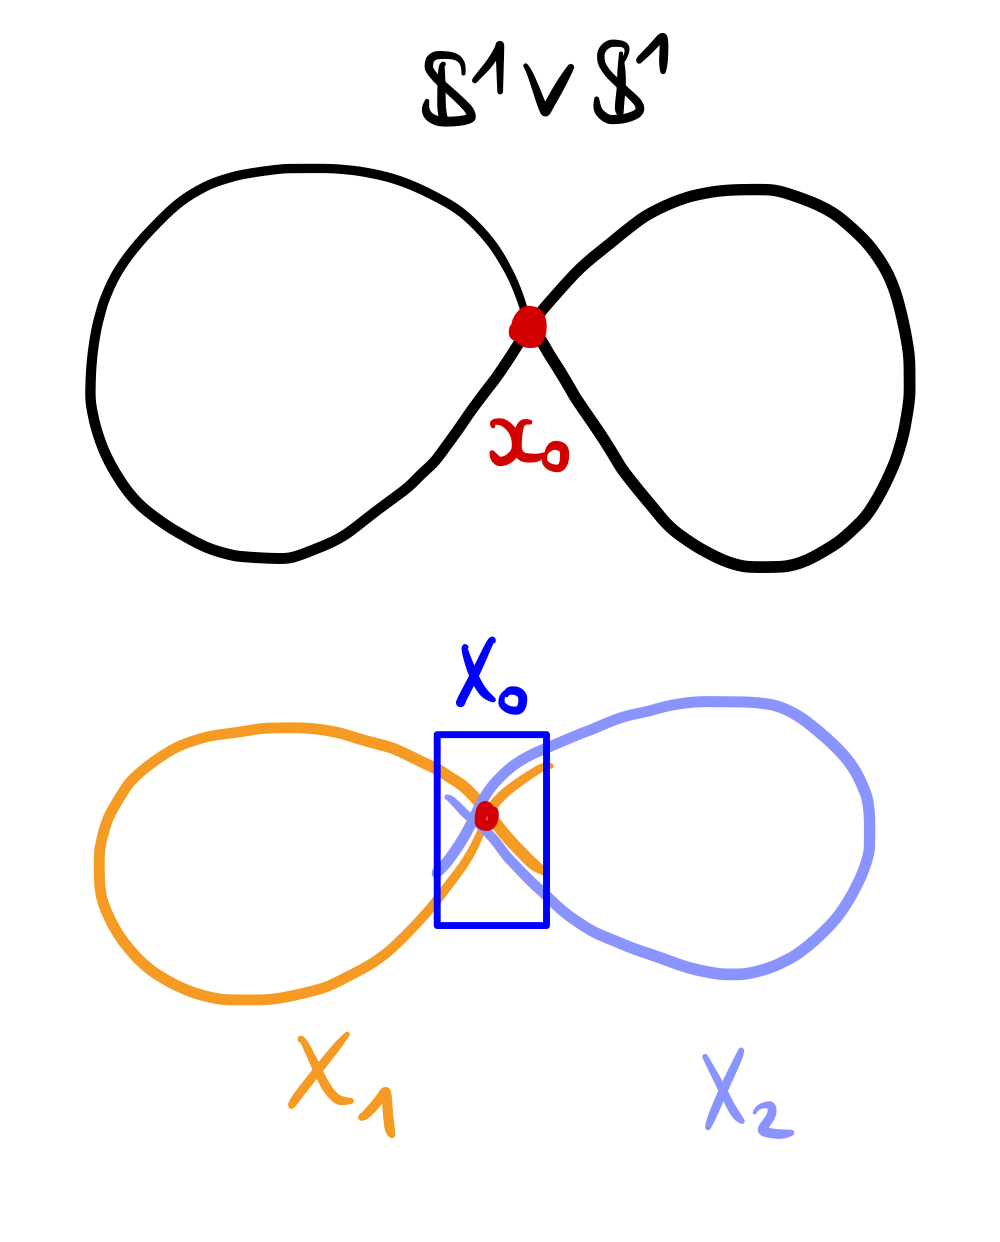
\includegraphics[scale=.08]{figures/wedge.png}
        \caption{We take $X_1$ and $X_2$ to be circles with little overlapping open tails. Those open tails retract onto the circles and do therefore not influence the fundamental group. The overlap is a small, open, x-shaped set which retracts onto a point and hence has trivial fundamental group.}
        \end{marginfigure}
    \begin{itemize}
        \item Consider again the connected sum of two circles (figure $8$): We cover the left and the right circle respectively with circles with small overlap, see the figure. We know that $\pi_1(\mathbb{S}^1)\cong \mathbb{Z}$, and the overlap retracts onto a point, so $\pi_1(X_0,x_0) \cong \{0\}$. This is a proof of our previous statement $$\pi_1(\mathbb{S}^1 \vee \mathbb{S}^1) \cong \mathbb{Z} \star_{0} \mathbb{Z} \cong \mathbb{Z} \star \mathbb{Z}.$$
        \item The previous result is very useful: Looking at the picture, you can see that the punctured Klein flask $K \setminus \{x\}$ is a retract of $\mathbb{S}^1 \vee \mathbb{S}^1$ and hence $\pi_1(K\setminus \{x\}) \cong \mathbb{Z} \star \mathbb{Z}$.
    \end{itemize}
\end{eg}
We want to illustrate the general principle of how to use Seifert-van Kampen with fundamental polygons with an example.
\begin{prop}
    The fundamental group of the Klein bottle $K$ is given by
    $$\pi_1(K, x_0)\cong \mathbb{Z} \rtimes \mathbb{Z} \cong \langle a,b \mid abab^{-1} \rangle.$$
\end{prop}
\begin{proof}
    \begin{marginfigure}
        \centering
        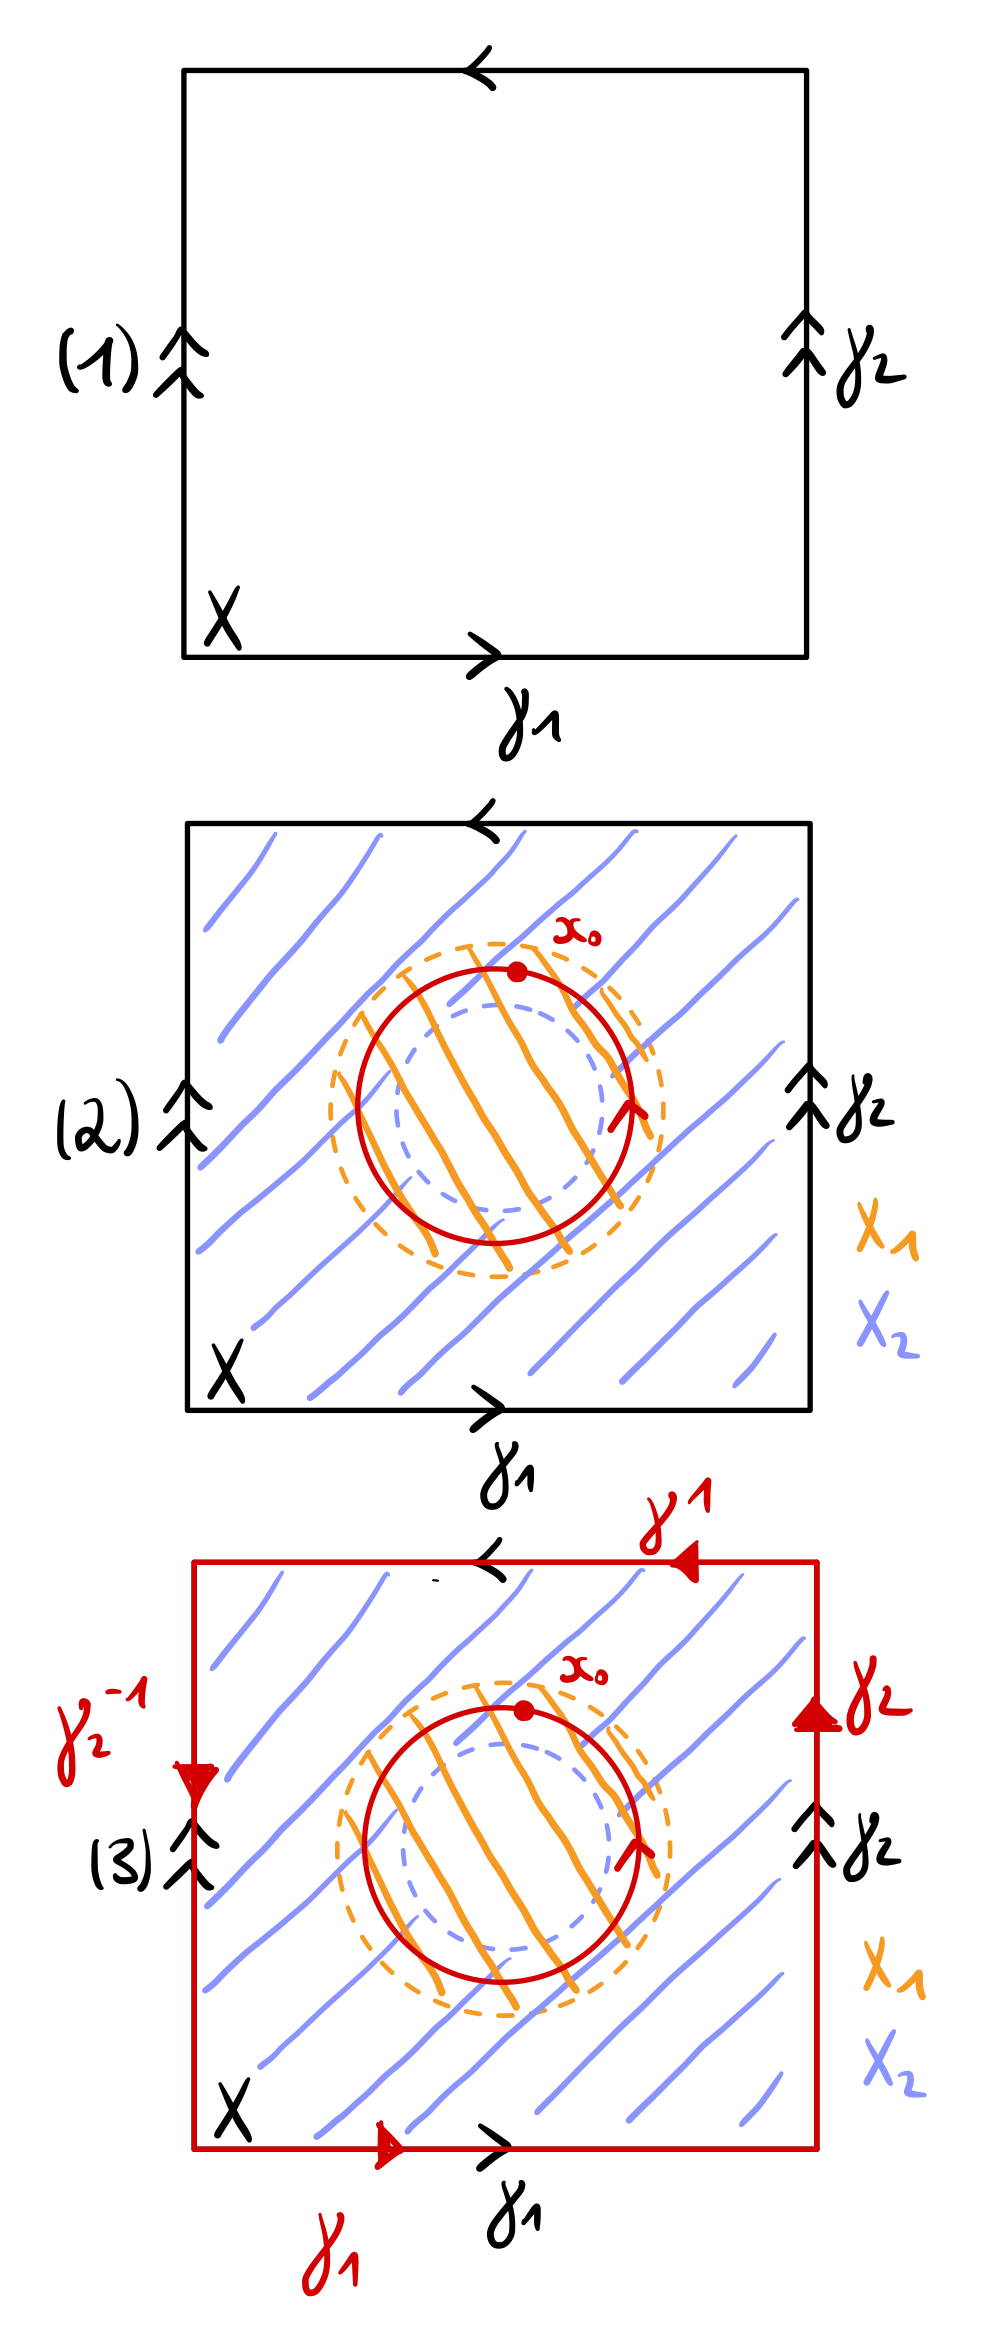
\includegraphics[scale=0.1]{./figures/klein.png}
    \end{marginfigure}
    We follow the picture in the margin:
    \begin{enumerate}
        \item Start by drawing the fundamental polygon of the Klein bottle and assign to each path generating the fundamental group a name, here $\gamma_1$ and $\gamma_2$. 
        \item Choose $X_1$ to be a small open disk in the middle of the polygon. Choose $X_2$ to be everything but a smaller closed disk in the middle, so that $X_2$ is open too. Choose some $X_0$ in the intersection of $X_1$ and $X_2$.
        \item We embed the subsets $\iota_1: X_1 \hookrightarrow X$ and $\iota_2: X_2 \hookrightarrow X$. This induces homomorphisms $\iota_{1,\ast}, \iota_{2,\ast}: \pi_1(X_i) \rightarrow \pi_1(X)$. These homomorphisms are the ones we need for the amalgamated product. Now choose a path in $X_0$ going through $x_0$ and traverse the fundamental polygon once in the chosen direction. When you first pass a generator, write the generator down with a positive sign if you go in the same direction or with a negative sign else.
    \end{enumerate}
    This is all we need. Now we calculate the needed fundamental groups: The open disk is simply connected, so $$\pi_1(X_1) \cong \{0\}$$ and we get no relations from this one. .\marginnote{Note how the notation for amalgamation $G_1 \star_{H} G_2$ suppresses very important information as the amalgamation depends heavily on the maps $\iota_i: G_i \to H$ not mentioned in this notation. Actually, if this were not the case, the fundamental group of the Klein bottle would agree with that of the torus.} The overarching set $X_2$ has two generators, so it is the free group on two generators $$\pi_1(X_2) \cong \langle \gamma_1, \gamma_2 \mid \emptyset \rangle.$$ Now the interesting part: $X_0$ is a so-called open annulus which retracts onto $\mathbb{S}^1$ and hence $$\pi_1(X_0) \cong \mathbb{Z}$$. But we have to be careful: The amalgamation forces the embedded red path to agree with the two generators on the boundary. Traversing the boundary once, this forces $\gamma_1 \gamma_2 \gamma_1 \gamma_2^{-1} = 1$, and hence
    $$ \pi_1(K) \cong \{0\} \star_{\mathbb{Z}} \mathcal{F}_2 \cong \langle \gamma_1, \gamma_2 \mid \gamma_1 \gamma_2 \gamma_1 \gamma_2^{-1}\rangle.$$
\end{proof}
Now we want to tackle our real problem.
    \begin{marginfigure}
        \centering
        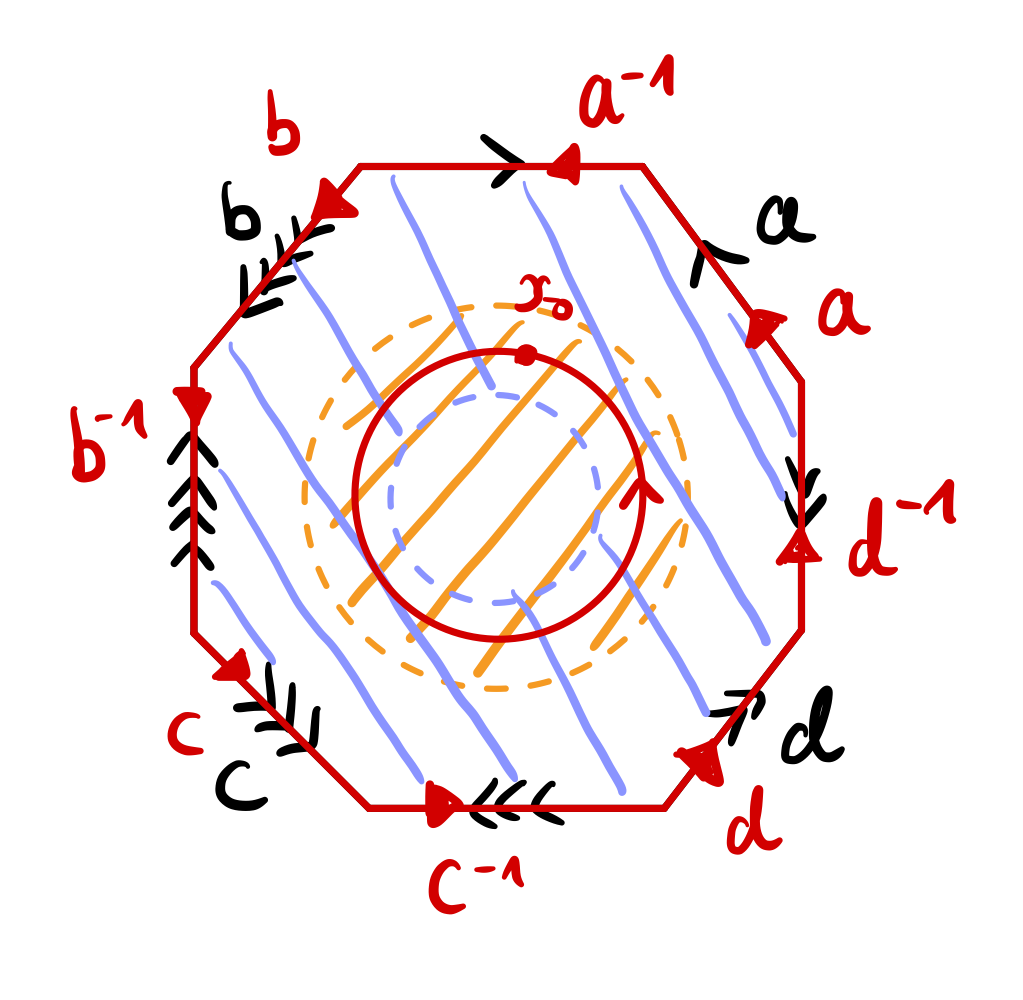
\includegraphics[scale=.15]{figures/problem}
    \end{marginfigure}
\begin{prop}
    The fundamental group of the top. space given by the fundamental hexagon on the left is
    \begin{equation}
        \pi_1(X) \cong \mathbb{Z} \ast \mathbb{Z} \ast \mathbb{Z} \ast \mathbb{Z} \cong \mathcal{F}_4.
    \end{equation}
\end{prop}
\begin{proof}
   Same game as above, choose $X_1$, $X_2$ and $X_0$ accodingly. In this case, $\pi_1(X_2)$ is the free group on four generators, $\langle a,b,c,d \mid \emptyset \rangle$. The fundamental group of $X_1$ and $X_0$ are still the same. The embedding of a path in $X_0$ traverses generators in the following way:
   $$aa^{-1}bb^{-1}cc^{-1}dd^{-1}.$$
   By Seifert-van Kampen, we obtain:
   \begin{equation}
       \pi_1(X) \cong \{0\} \star_{\mathbb{Z}} \mathcal{F}_4 \cong \langle a,b,c,d \mid aa^{-1}bb^{-1}cc^{-1}dd^{-1}\rangle.
   \end{equation}
   But we are always allowed to reduce mutually inverse elements, so the relation reduces to $1=1$, the trivial relation. So we just get the free group on four generators again.
\end{proof}
Note that this means that our space is homotopy equivalent to the wedge sum of four circles $\mathbb{S}^1 \vee \mathbb{S}^1 \vee \mathbb{S}^1 \vee \mathbb{S}^1$.

